
\documentclass[submit, techrep]{ipsj}
%\documentclass{ipsj}

\usepackage[dvipdfmx]{graphicx}
\usepackage{latexsym}
\usepackage{color}
\usepackage{amsmath}
\usepackage{siunitx}

\input{00_macro}

\def\Underline{\setbox0\hbox\bgroup\let\\\endUnderline}
\def\endUnderline{\vphantom{y}\egroup\smash{\underline{\box0}}\\}
\def\|{\verb |}


\setcounter{巻数}{59}
\setcounter{号数}{1}
\setcounter{page}{1}

\makeatletter
\pagestyle{empty}
\def\@oddhead{}%
\def\@evenhead{}%
\def\ps@IPSJTITLEheadings{}
\makeatother







\begin{document}


\title{距離センサアレイを用いた膝によるカーソル操作手法}



\affiliate{CS1}{筑波大学 システム情報工学研究科 \\コンピュータサイエンス専攻}
\affiliate{CS2}{筑波大学 システム情報系}


%\paffiliate{JU}{情報処理大学\\
%Johoshori University}

\author{市川 佑}{}{CS1}[yichikawa@iplab.cs.tsukuba.ac.jp]
\author{志築 文太郎}{}{CS2}[shizuki@cs.tsukuba.ac.jp]
\author{高橋 伸}{}{CS2}[shin@cs.tsukuba.ac.jp]

\begin{abstract}
本研究では,机裏に設置した距離センサアレイにより,膝の位置を認識し,カーソル操作に応用することを提案する.
ユーザは机の前に座り,机の下で膝を上下左右に動かすと,カーソルを操作できる.
これはキーボードなどの手による操作と並行して行うことができる.
机の裏に機器を設置することにより,ユーザの邪魔になりにくく,身体に装置を取り付ける必要もない.
我々は.距離センサアレイを製作し,膝の位置の認識,膝の位置からカーソル座標への変換を行うシステムを実装した.
システムは簡単なキャリブレーションを行うことで,様々な体格の人に対応させることができる.
我々はシステムをカーソル操作に適用し実験を行い,膝の操作性やユーザの疲労感,上下左右方向への膝の運動の難易を調査した.
%さらに,膝による操作の応用例として、一人称視点ゲームへの適用を提案する.
\end{abstract}






\maketitle

%1
\section{背景}
様々なペダルの操作に代表されるように,我々は日常的に足による操作を行なっている.
しかし,パーソナルコンピュータやスマートフォンを操作する際,我々は手を中心に操作を行い,足に操作が割り当てられることはなく,ほとんど動かすことがない.
足による操作を用いたコンピュータ向けインタフェースの研究は,1960 年代から存在している\cite{1698228}が,現在は手による操作が中心である.
しかし,手がふさがった状態における機器の操作\cite{Fan:2017:ESF:3123021.3123043}など,足によるインタラクションの研究は関心が高まっている.\par
机上でコンピュータを用いる作業では両手をキーボードの操作に充てることが多い.
足によってマウスカーソルの操作を行うことで,両手はキーボード操作を行ったまま,マウスカーソルの制御が可能になる.
先行研究には装置を足で動かす方法\cite{Pearson:1986:MMD:22627.22392, Pearson:1988:EEP:57167.57169}や,足の位置によって摩擦力を変えることができる機構を取り付けた靴\cite{Horodniczy:2017:FHE:3025453.3025625}を用いる方法がある.
これらは体の一部に装置を取り付けるあるいは大型な装置を用いるものであるため,ユーザの衣服などに制限が生じる,装置を持ち運ぶことができないといった制約が存在する.\par
本研究では膝の位置を読み取る装置を開発し,これを机の下に取り付けることで,認識した膝の位置をマウスカーソルの操作に適用することを行う.
これにより,特別な装置を足に装着することなく,かつ小型な装置で,足を用いたコンピュータの操作を可能とした.
膝を使う理由は 2 点ある.
1点目に,膝は足先と比べてより自由な操作が行える可能性がある.2点目に,膝と足による操作の組み合わせによりさらなるインタラクションの拡張が可能である.

\section{関連研究}
\subsection{足によるジェスチャ入力}
足による入力に焦点を当てている研究では,まず足のジェスチャを用いるものが挙げられる.
まず,屋外でスマートフォンなどを操作する時に荷物を持っている,手が汚れているというすぐに手を用いることができない状況を想定した研究を挙げる.
Fanら\cite{Fan:2017:ESF:3123021.3123043}は,足のジェスチャによりモバイル端末を操作することに対する実証研究を行なった.
ユーザ定義の足のジェスチャを用いた方法と,荷物を降ろして手で端末を持ち操作する方法を比較したところ,前者の方が70\%高速な操作が可能であるという結果となった.
HanらのKick\cite{Han:2011:KIU:2037373.2037379}では,蹴り出すジェスチャを端末操作に用いるために,ユーザがキックの方向と速度をどの程度制御できるかを調査した.
本研究は,屋内での利用のみを想定した環境設置型の装置を用いるという点と,ラップトップコンピュータやデスクトップコンピュータへの利用を想定しているという点から,インタラクションの目的は異なる.\par
また,屋内環境を想定して装置を設置することでインタラクションを実現した例として,AugstenらによるMultitoe\cite{Augsten:2010:MHI:1866029.1866064}では,巨大なタッチパネルを床面に設置し,複数の足の認識や足の重心位置の認識した.
これにより,床面に表示されたメニューやキーボードを足で操作することを提案した.
この研究では立った状態を想定しているが,本研究では,デスクトップ上での作業中という限定された環境におけるインタラクション手法の提案を目指す.


\subsection{机上での作業における足を使ったコンピュータ操作}
机上におけるコンピュータの操作に足を用いた入力手法を調査,提案した研究例を挙げる.
Saundersら\cite{Saunders:2016:TFI:2901790.2901815}は,立った状態でのデスクトップアプリケーションの制御に足を用いた.
Pearsonら\cite{Pearson:1986:MMD:22627.22392, Pearson:1988:EEP:57167.57169}は「モル」という装置を開発し,ポインタの操作などに手の代わりに足を使用する方法を調査した.モルを用いた場合でも,訓練によって小さなターゲットを選択することが可能になることを示した.
Horodniczyら\cite{Horodniczy:2017:FHE:3025453.3025625}は,ユーザの靴に可変摩擦式の装置を取り付け,足によるカーソル操作の補助装置として用いた.靴底には低摩擦材と高摩擦材の2つを取り付け,高摩擦材の接地圧力をステッピングモータで制御する.足の位置をカメラにより取得し,ターゲットに近づくにつれ圧力を高める.
Vellosoら\cite{velloso:hal-01599657}は,座っている状態の机の下の足の動きの特徴を調査した.机の下に配置したカメラから,片方の足のつま先をマウス操作に割り当て,1次元と2次元におけるポインティング作業により,パフォーマンスのテストを行なっている.
これらの研究では,大型の装置を用いているために持ち運びや設置が困難であったり,靴に対して装置を取り付けるためにユーザに身体上の制約を強いてしまう.
本研究では小型で設置が簡単かつ足に装置を取り付けないアプローチで,問題の解決を図る.
また,本研究は足先でなく膝に焦点を当てることで,既存手法との組み合わせによってさらなるインタラクションの拡張を図ることも可能である.\par
足と他の入力モダリティとの組み合わせを行なった研究という点では,次のようなものが存在する.
G\"{o}belら\cite{Gobel:2013:GFI:2468356.2479610}が提案する手法では視線と足を組み合わせ,視線位置におけるパンとズームの操作を足によるペダル操作で行うことを提案した.
Rajanna\cite{Rajanna:2016:GFI:2876456.2876462}は,視線によるポインティングと足によるクリックコマンドで構成されるシステムを構築した.
本研究では膝による入力操作を行うことで,足を用いた他の手法との組み合わせの可能性を探る.

\subsection{膝を用いたコンピュータへの入力}
膝に関する研究の中で,コンピュータへの入力を想定したものは少ない.
Englishら\cite{1698228}は,テキスト選択において,膝を含めたいくつかの装置やデバイスを用いた時の操作時間を調査した.
調査の結果,膝による操作は最も短い時間で選択することができることがわかった.
この論文では,机の下に取り付けた装置のレバーを膝で動かすことで入力を行なったが,この装置は調査を行うために作られた原始的なものであった.
本研究では,距離センサを使うことで,設計の工夫を行っている.

\section{膝によるコンピュータ操作の設計}
マウスやタッチパッドの操作と異なり,膝は前方や後方に動かすことはできない.
そのため,本研究で想定する膝の移動は,膝を傾けることによる左右方向と,かかとを浮かせたり床につけたりすることによる上下方向の移動である.
\refImg{knee_howto}は,ユーザが膝をどのように動かすかを表したイメージである.
\img{tb}{1}{sousa_overview.pdf}{カーソルの位置に対するユーザの膝のイメージ}{knee_howto}

マウスカーソルを左右に移動する時には,膝を左右に傾ける.
上方向に移動する時は,かかとを浮かせて膝を机に近づける.
逆に下方向に移動する時は,足を手前に引き,その時に浮いたかかとを床に近づけることで,膝を机から遠ざける.
足が完全に地面についている時にカーソルが真ん中にあるため,ユーザは比較的楽な姿勢で操作することができる.

\section{プロトタイプシステムの実装}
プロトタイプシステムは,三角法を用いた光学式距離センサ 10 個を一列に並べたセンサアレイ,マイコン,パーソナルコンピュータからなるハードウェアと,センサから距離データを取得し,膝の位置の認識,キャリブレーションの記録,カーソル座標への変換を行うソフトウェアからなる.
システムの処理の流れを\refImg{system_overall}に示す.
まず距離センサアレイからマイコンが距離データを取得する.マイコンは10個の距離センサそれぞれの計測値を1フレームにまとめる.PC上のプログラムでは,USBシリアル通信を通して舞い込んから距離データを取得する.\par
取得した距離データから膝の位置が計算される.本システムではキャリブレーションを行い,膝の可動範囲を記録する(\refImg{system_overall}の赤矢印).
この記録をもとに,膝の位置を画面上のカーソル座標へ変換する(\refImg{system_overall}の緑矢印).

\img{tb}{1.0}{system_overall.pdf}{プロトタイプシステムの全体図}{system_overall}

\subsection{距離センサアレイ}
距離センサは,SHARP社製GP2Y0E03を用いている.
この距離センサは三角測量の原理を用い,対象までの距離を計測する.
長さ約 30cm のプラスティック製の定規に,センサ本体を 30mm 間隔で定規に接着剤を使って固定した.
距離センサの向きは,GP2Y0E03 のアプリケーションノートに,距離を計測する移動物体に対するセンサの向きに関する記述があったため,横向きとなっている.\par
マイコンは10個のセンサが測定した距離を1フレームの距離データとして,USBシリアル通信を用いてPCに送信する.

\img{htbp}{1}{distance_sensor_array.pdf}{距離センサアレイ}{distance_sensor_array}

\subsection{膝の位置の認識とカーソル操作への適用}
\subsubsection{膝の位置の認識}
我々は,Xiao\cite{Xiao:2018:LOP:3173574.3173669}らの方法を参考に,距離データから膝の位置の計算と,PC画面上のカーソル座標への変換を行った.
%まず,取得した距離データを指数移動平均フィルタにかける.本システムでは,調整の結果平滑化係数$\alpha=0.1,0.65$の2種類のフィルタを使用している.時間$t$において取得した距離データ$d^t$に対して,フィルタリング後の距離データ$D^t$を\refEq{filter} のように計算する.
%\begin{eqnarray}
%	\label{eq:filter}
%	D^t = \alpha (d^t - D^{t-1}) + D^{t-1}
%\end{eqnarray}
%得られた$D^t$から,以下の手順で仮の膝の座標$K^t=(K^t_x, K^t_y)$を計算する.\\
取得した距離データを$D^t$として,以下の手順で仮の膝の座標$K^t=(K^t_x, K^t_y)$を計算する.まず、$k^t=(k^t_x, k^t_y)$を求め、最後に$k^t$を指数移動平均フィルタにかけて$K^t$を求める。
\begin{enumerate}
	\item $k^t_y$を$D^t$の最小値とする.
	\item i番目の距離センサについて,重み$w_i$を\refEq{weight}のように計算する.$d$は重みを調整するための定数であり,本システムでは調整の結果$d=2$としている.
	\begin{eqnarray}
		\label{eq:weight}
		w_i = \frac{1}{D^t_i - k^t_y + d}
	\end{eqnarray}
	\item $w_i$から$k^t_x$を\refEq{calc_x}のように計算する.
	\begin{eqnarray}
		\label{eq:calc_x}
			k^t_x = \frac{\Sigma_i iw_i}{\Sigma_i w_i}
	\end{eqnarray}
	\item $k^t$を指数移動平均フィルタにかける.ここでは、$\alpha=0.7$としている.
\begin{eqnarray}
	\label{eq:filter}
	K^t = \alpha (k^t - K^{t-1}) + K^{t-1}
	\end{eqnarray}
\end{enumerate}
\subsubsection{カーソル座標への変換}
本システムでは,膝の位置をカーソル座標へ変換するには,キャリブレーションを必要とする.
キャリブレーションは膝の上下左右の可動域と中心位置に対して行う.
可動域はユーザが膝を動かすことができる限界ではなく,任意に決定することができる.
これにより,画面を4つの領域に分けてそれぞれ異なるCD値として,操作をより簡単にすることを図っている.
キャリブレーションによって,左右の可動域における$K^t_x$,上下の可動域における$K^t_y$,中心位置における$(K^t_x, K^t_y)$を記録する.
以降は,記録した上下左右の4点を$(C_{left},C_{right},C_{upper},C_{lower})$,中心位置を$C_{center}=(C_{center_x},  C_{center_y})$と表す.\par
キャリブレーションの記録から,画面上のカーソル座標$(P_x, P_y)$を\refEq{calc_px},\refEq{calc_py}のように計算する.
ここでは,解像度が$(W_x, W_y)$であるディスプレイを想定している.
\begin{eqnarray}
	\label{eq:calc_px}
	P^t_x = 
	\begin{cases}
		\frac{(K^t_x - C_{left}) \left( \frac{W_x}{2} \right)}{C_{center_x} - C_{left}} & (K^t_x < C_{center_x})\\
		\frac{(K^t_x - C_{center_x}) \left( \frac{W_x}{2} \right)}{C_{right} - C_{center_x}} & (C_{center_x} \leq K^t_x)
	\end{cases}	 
\end{eqnarray}
\begin{eqnarray}
	\label{eq:calc_py}
	P^t_y = 
	\begin{cases}
		\frac{(K^t_y - C_{upper}) \left( \frac{W_x}{2} \right)}{C_{center_y} - C_{upper}} & (K^t_y < C_{center_y}) \\
		\frac{(K^t_x - C_{center_y}) \left( \frac{W_x}{2} \right)}{C_{lower} - C_{center_y}} & (C_{center_y} \leq K^t_y)
	\end{cases}
\end{eqnarray}
\section{評価実験}
本プロトタイプシステムを用いて評価実験を行い、膝によるマウスカーソル操作の性能と、ユーザが感じる膝の操作の難易、疲労感を調査する。加えて、膝の方向によって性能に差があるかを調査する。
実験にはISO9241-411\cite{9241411}に記載されている,マルチディレクショナルポインティングタスクに基づいて実装したプログラムを用いた。\refImg{mdpt}はそのプログラムである。
\begin{figure}[tb]
	\begin{center}
		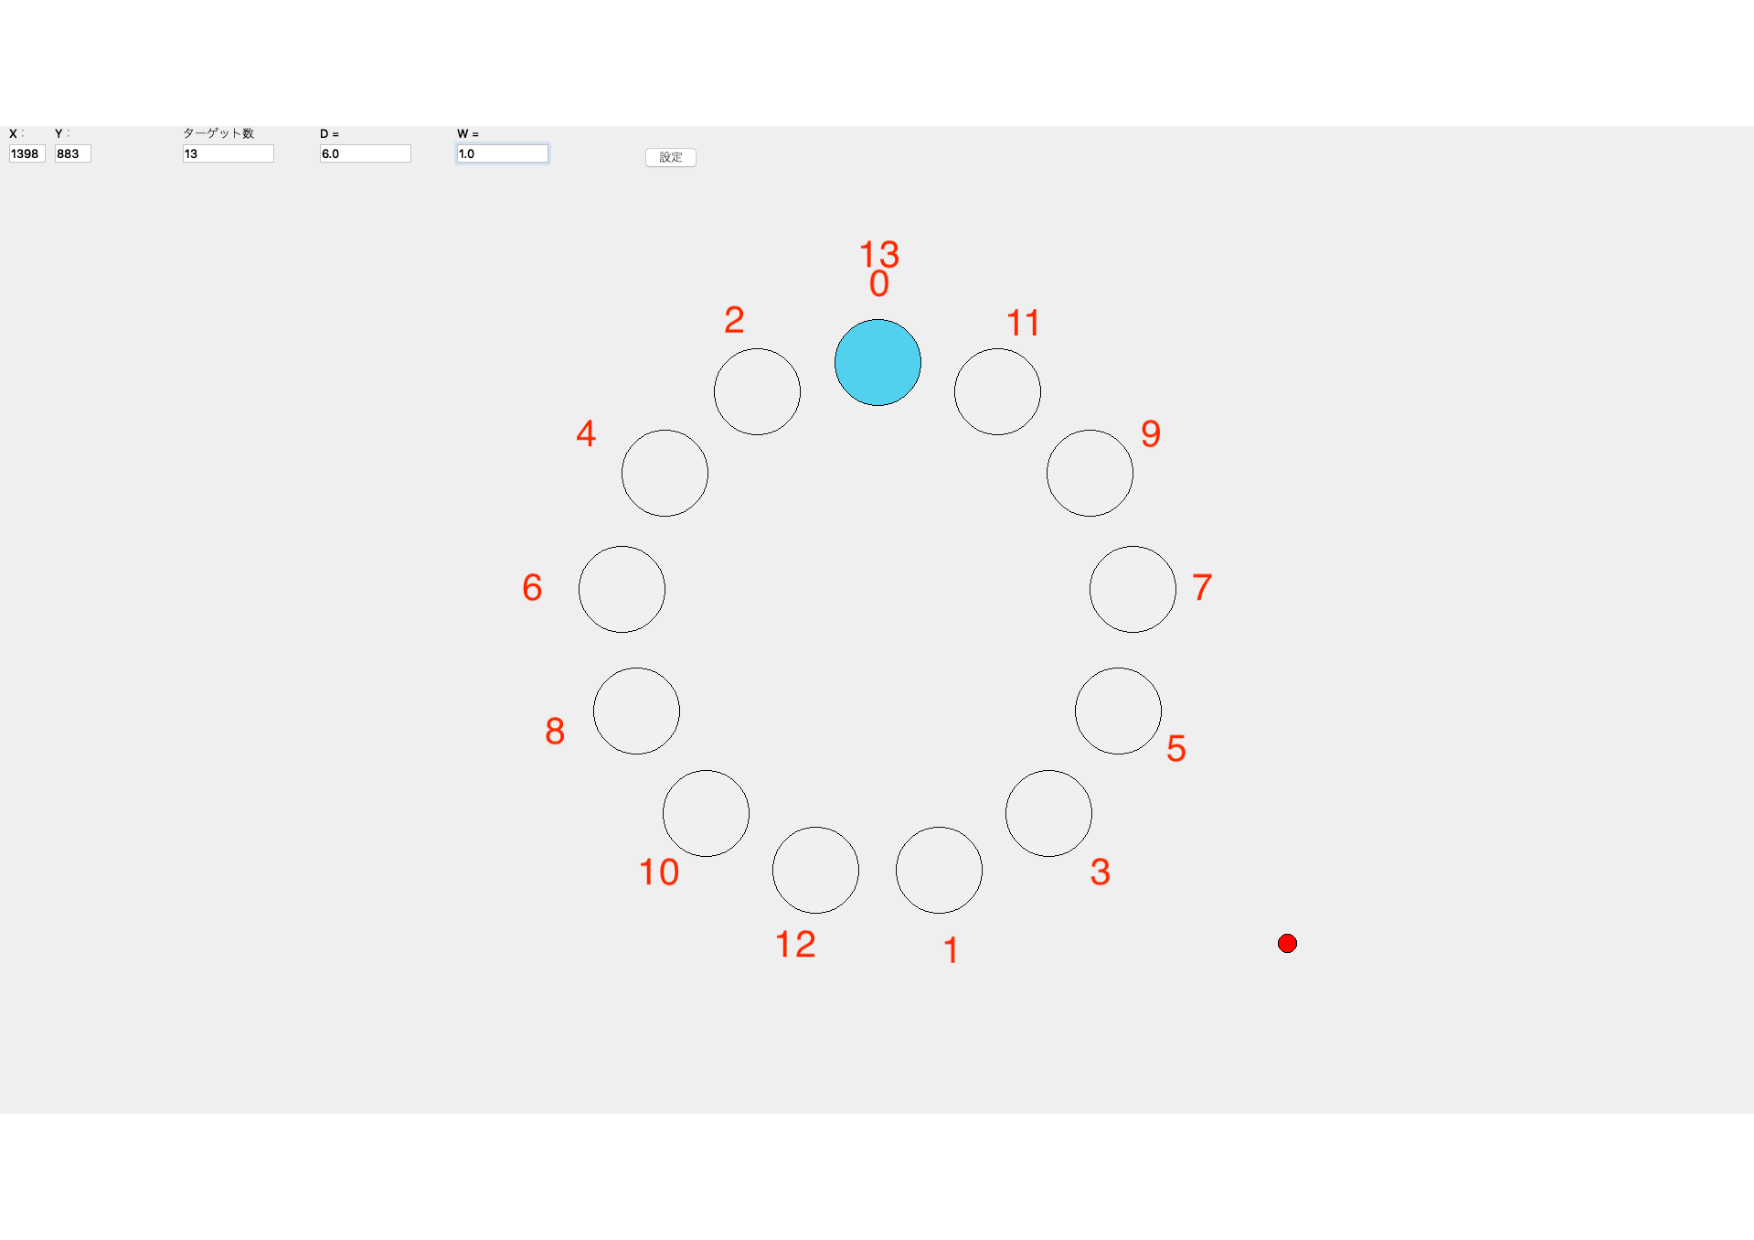
\includegraphics[angle = 270, width = 1.0\hsize]{./figures/1.pdf}
	\end{center}
	\caption{実験に使用したプログラムの画面}
	\label{img:mdpt}
\end{figure}
%\img{htbp}{1.0}{1.pdf}{実験に使用したプログラムの画面}{mdpt}
\subsection{評価方法}
評価にはフィッツの法則\cite{fitts}を用いる。
フィッツの法則は\ref{eq:fitts}で表される。
\begin{eqnarray}
	MT = a + b\log_2{(D/W + 1)}
	\label{eq:fitts}
\end{eqnarray}
$MT$とはカーソルをターゲットに移動させるまでにかかると想定される時間である。
$a$と$b$は実験環境や機器に依存する定数である。
$D$はターゲット間の距離、$W$はターゲットの大きさ(円の直径)を表す。
なおこの実験では、$D$はターゲットが配置されている円周の直径としている。
また、$\log_2{(D/W + 1)}$という式はIndex of Difficulty(ID)とも呼ばれ、課題の困難度を表す指標である。
本研究では、Soukoreffら\cite{Soukoreff:2004:TSP:1056153.1056155}によって示されている方法を参考に、$D_e$,$W_e$および$ID_e$について計算を行い評価を行う。
\subsection{実験条件}
\subsubsection{ターゲットサイズ}
実験条件は、$D$と$W$を次のように変化させる。
\begin{itemize}
	\item {D: } 3.0, 15.0, 26.0 \si{cm}
	\item {W: } 0.8, 1.8, 2.4 \si{cm}
\end{itemize}
これにより、9種類の$ID$の値 \{1.170, 1.415, 2.248, 2.858, 3.222, 3.565, 3.949, 4.304, 5.066\}を得る。

\subsubsection{実験手順}
実験参加者は水色の円で示されるターゲットに、赤色の円で示されるカーソルを膝で操作し、2つが重なったときに選択操作を行う。
この選択操作1回を1試行と数える。
なお選択操作は足ではなくキーボード上のEnterキーで行う。
\refImg{mdpt}に示されている番号$0,1,...,13$の順に14試行を行う。ただし、$1,2,...,13$番の選択についてのみ実験データとして記録を行い、$0$番の選択は記録しない。\par
はじめ、ターゲットは全てオレンジ色で表示されている。
実験参加者がCommandキーを押すことで、実験が開始され、ターゲットを選択できるようになる。
13試行を終えると、再びターゲットはオレンジ色で表示される。
このとき、Shiftキーを押すことで、実験条件が変化する。
9条件すべてについて実験を行うことを1セッションと数える。
セッションの中で条件はランダムな順番で切り替わる。
実験は左膝、右膝について5セッションずつ行う。どちらかの膝について5セッション行うことを1ピリオドと数える。
第1ピリオドの終了後に5分間の休憩を設けた。
\subsubsection{実験機器}
実験に用いる機器は、ディスプレイ(DELL S2409Wb 24inch 1920*1080)、コンピュータ(Apple MacBookPro 2018 TouchBar)、プロトタイプシステム、外付けキーボード(Apple Magic Keyboard 2)である。
$D$と$W$の大きさは、ディスプレイの実寸と解像度を元にプログラム内でピクセル値に変換されている。
%また、ノイズを軽減するため距離センサの真下に白いシートを敷いた。実験参加者は靴を脱いだ状態で足をシートに乗せて操作を行う。
\subsubsection{収集データ}
解析のために、実験参加者が1回の試行に要した時間、選択おいてミスをしたかを表すフラグ、1試行における操作の開始点と終点およびターゲットとして表示されている円の中心座標を収集した。
参加者1人あたりのデータ数は、$13$(試行)$*9$(ターゲットサイズ条件)$*5$(セッション)$*2$(左右膝)$ = 1170$である。
\subsection{アンケート}
実験の最後にアンケートを行い、参加者の疲労感と膝によるコンピュータ操作の難易について調査した。
疲労感については以下の4項目を5点リッカート尺度で評価してもらった(1-全く疲れていない、5-とても疲れている)。
\begin{itemize}
	\item {Q1: }太ももの疲労感
	\item {Q2: }ふくらはぎの疲労感
	\item {Q3: }足先の疲労感
	\item {Q4: }精神的な疲労感
\end{itemize}
加えて、項目になかった体の部位で疲れている箇所を自由記述形式で記述してもらった(Q5)。
膝によるコンピュータ操作の難易については、以下の2項目を5点リッカート尺度で評価してもらった。
\begin{itemize}
	\item {Q6: }膝による操作は意図した通りに行うことができたか(1-全く行うことができなかった、5-とても行うことができた)。
	\item {Q7: }膝を無理に動かさなければならない操作があったか(1-全く当てはまらなかった、 5-全て当てはまる)。
\end{itemize}
加えて、膝による操作で簡単であった点、難しかった点を自由記述形式で記述してもらった(Q8)。
\subsection{実験参加者}
実験参加者は4名である。
年齢の内訳は22歳が1名(P3)、23歳が3名(P1,P2,P4)であり、全員が男性の大学院生である。
順序効果を除くために、P1とP3は左膝、右膝の順に、P2とP4は右膝、左膝の順に実験を行なった。
実験開始前に足の大腿と下腿の長さを測定した。
結果を\refTb{length}に示す。(単位は\si{cm})
\begin{table}[tb]
	\begin{center}
		\begin{tabular}{|c|c|c|c|c|}
		\hline
			& P1 & P2 & P3 & P4 \\ \hline
		大腿 & 37 & 35 & 38 & 42 \\ \hline
		下腿 & 48 & 40 & 42 & 38 \\ \hline
		\end{tabular}
	\end{center}
	\caption{参加者ごとの大腿と下腿の長さ}
	\label{tb:length}
\end{table}
\subsection{結果}
\subsubsection{カーソル操作の性能}
\refImg{graph_raw}は、それぞれ左膝、右膝における実験結果である。縦軸が選択時間、横軸が実験結果から計算された$ID_e$を表す。
\img{tb}{1.0}{graph_raw.png}{左右膝の選択時間と線形回帰モデル}{graph_raw}
\refImg{error_rate}は左右の膝におけるターゲット選択のエラー率を表している。各参加者ごとのエラー率がセッションごと、5セッションの平均で示されている。全参加者のエラー率の平均は、左膝で$9.15\%$、右膝で$10.86\%$であった。
\img{tb}{1.0}{error_rate.png}{左右膝の選択時エラー率}{error_rate}
\refImg{tp}は、参加者ごとと全参加者の平均のスループットを表している。全参加者の平均のスループットは、左膝が$1.93[bit/s]$、右膝が$1.69[bit/s]$であった。
\img{tb}{0.85}{tp.png}{左右膝のスループット}{tp}
\subsubsection{膝の移動方向別の結果}
我々は、カーソルの移動方向が水平方向か垂直方向かで、性能が異なるかを調査した。\refImg{mdpt}において、水平方向の移動は選択ターゲットが6,7,8の時、垂直方向の移動は0,1,12,13の時と定義した。
\refImg{direction}は水平方向の移動、垂直方向の移動のみを取り出した実験結果である。縦軸が選択時間、横軸が実験結果から計算された$ID_e$を表す。
\img{tb}{1.0}{direction.png}{方向別の選択時間と線形回帰モデル}{direction}
\refTb{err_direction}は移動方向別のエラー率を表している。LはLeft Knee、RはRight Kneeを表し、HはHorizontal、VはVerticalを表す。すなわち、(L,H)はLeft KneeのHorizontalの移動を表す。
\begin{table}[tb]
	\begin{center}
		\begin{tabular}{|c|c|c|c|c|}
		\hline
				& P1 & P2 & P3 & P4 \\ \hline
		(L, H) & 7.41\% & 18.5\% & 4.44\% & 7.41\% \\ \hline
		(L, V) & 2.22\% & 20.0\% & 6.67\% & 6.67\% \\ \hline
		(R, H) & 8.89\% & 17.8\% & 15.6\% & 6.67\% \\ \hline
		(R, V) & 2.22\% & 15.6\% & 20.6\% & 5.00\% \\ \hline
		\end{tabular}
	\end{center}
	\caption{方向別のエラー率}
	\label{tb:err_direction}
\end{table}
\refTb{tp_direction}は、移動方向別に計算したスループットである。
\begin{table}[tb]
	\begin{center}
		\begin{tabular}{|c|c|c|}
		\hline
				   & Horizontal & Vertical   \\ \hline
		Left Knee  & 1.90 & 2.32  \\ \hline
		Right Knee & 1.54 & 1.97  \\ \hline
		\end{tabular}
	\end{center}
	\caption{方向別のスループット}
	\label{tb:tp_direction}
\end{table}

\subsubsection{アンケート結果}
\refTb{quest}はアンケートの中で、リッカート尺度で評価された部分における結果である。
\begin{table}[tb]
	\begin{center}
		\begin{tabular}{|c|c|c|c|c|c|}
		\hline
		   & P1 & P2 & P3 & P4 & Average \\ \hline
		Q1 & 4 & 4 & 2 & 4 & 3.50\\ \hline
		Q2 & 3 & 3 & 2 & 4 & 3.00\\ \hline
		Q3 & 2 & 4 & 2 & 3 & 2.75\\ \hline
		Q4 & 4 & 5 & 3 & 3 & 3.75\\ \hline
		\hline
		Q6 & 4 & 4 & 3 & 4 & 3.75\\ \hline
		Q7 & 2 & 2 & 2 & 3 & 2.25\\ \hline
		\end{tabular}
	\end{center}
	\caption{リッカート尺度で評価された部分のアンケート結果}
	\label{tb:quest}
\end{table}
Q5においては、腰(P1)、目(P4)に疲労感を感じたという意見を受けた。また、実験時間が長く思いの外疲れたので、休憩を増やして欲しかった(P3)という意見もあった。Q8においては、下方向のカーソル移動が難しい(P1,P3,P4)という意見があった。具体的には、足を引く動作において微調整が難しい(P3)、キャリブレーションの時より大きく動かさなければならない(P4)と述べた。

\subsection{議論}
左右の膝におけるスループットの値は、数値のみの比較では、Vellosoら\cite{velloso:hal-01599657}による足を用いたカーソル操作の結果より高いものであった。したがって、膝によるコンピュータ操作は足による操作より高速に行える可能性がある。一方でエラー率に関しては若干高い結果となった。特にP2の両膝における結果とP3の右膝において高い。これは、キャリブレーション時に上下の膝位置の差が小さく、小さな膝の動きに対してカーソルの移動量が大きくなってしまったことが考えられる。今後プロトタイプシステムの膝位置認識や座標計算の方法を見直すことで改善を図る。\par
移動方向別の分析では、スループットの面で水平方向よりも垂直方向の方が高い値を示した一方で、アンケートでは下方向の移動が難しいという意見が多かった。これは、左右方向の膝位置認識では全ての距離センサから送信されるデータを総合しているのに対し、上下方向には距離センサの最小値が膝位置となるので、より正確な位置となっていると考える。\par
アンケートではまた、膝による操作は比較的簡単で、参加者が行える範囲であることが読み取れる。

%\section{応用例:一人称視点ゲームにおける膝によるプレイヤー移動}
%本プロトタイプシステムの応用例として、一人称視点ゲームのプレイヤーを、膝を用いて前後左右に移動させることを提案する.PC上でプレイする一人称視点ゲームでは、一般にマウスを前後左右に動かすことで視点を上下左右に、キーボードでプレイヤーの移動方向を操作する.しかしキーボードとマウスを常に同時に操作するために,机上に大きなスペースが必要になるといった問題がある.プレイヤーの移動を膝で代用することにより、こうした問題を解決できるのではないかと考える.
%我々は、Unityを用いて\refImg{}のようなサンプルプログラムを実装した.膝の位置を認識し、片方の膝を上下左右に操作した時にプレイヤーが前後左右に移動するスクリプトを実装し、プレイヤーの移動を実現した.

\section{今後の展望}
実験時アンケートの結果では、太ももの疲労感が比較的高いことが読み取れる。左右方向の操作が膝を傾けるのみなのに対し、上下方向の操作はかかとを持ち上げる、手前に引くなど通常あまり行わない動作が多く、今後操作方法の見直しを行う。\par
現在のシステムでは、スカートといった、両膝が衣服によって接続されている場合に対応できない。対策として、膝にマーカなどを取り付けて、両膝を識別するなどを考えている。\par
また、今回はカーソルの移動のみであったが、スイッチを使用しない方の足で踏むことによるクリック操作の実現や、両膝を用いることでピンチ・パンといったジェスチャ操作の実装を目指す。\par
実験結果より、足による操作より単純な数値では速い操作ができる可能性があると分かったが、マウスの速度は3.7[bit/s]以上\cite{Soukoreff:2004:TSP:1056153.1056155}であるという結果があるため、操作方法やプロトタイプシステムの実装を見直すことで速度の改善を図る。

\section{結論}
本研究では膝の位置を、机の裏に設置した距離センサアレイによって認識するデバイスを開発した。
このデバイスは特別な装置を足に取り付ける必要がなく、装置がユーザの邪魔となりにくい。
我々は距離センサアレイから距離データを取得し、膝の位置を認識し、カーソル座標へ変換するプロトタイプシステムを実装した。
また、プロトタイプシステムを用いた実験では、単純な数値比較において足先によるカーソル操作より速度の面でよいという結果を得た。
さらに,VR一人称視点ゲームへの膝による操作の応用例の提案を行った.
今後はユーザの膝の動かし方や膝の位置の計算方法を見直すことで、速度とユーザの疲労感における改善を目指す。また、ユーザが様々な衣服を着用した場合の対応を行う。


%% bib
\bibliographystyle{ipsjunsrt-e}
%\bibliographystyle{ipsjsort}
%\bibliographystyle{junsrt}
%\bibliography{bibsample}
\bibliography{ref.bib}



\begin{biography}
\profile{m,E}{情報 太郎}{1970年生.1992年情報処理大学理学部情報科学科卒業.
1994年同大学大学院修士課程修了.同年情報処理学会入社.オンライン出版の研究
に従事.電子情報通信学会,IEEE,ACM 各会員.}
%
\profile{n}{処理 花子}{1960年生.1982年情報処理大学理学部情報科学科卒業.
1984年同大学大学院修士課程修了.1987年同博士課程修了.理学博士.1987年情報処
理大学助手.1992年架空大学助教授.1997年同大教授.オンライン出版の研究
に従事.2010年情報処理記念賞受賞.電子情報通信学会,IEEE,IEEE-CS,ACM
各会員.}
%
\profile{h,L}{学会 次郎}{1950年生.1974年架空大学大学院修士課程修了.
1987年同博士課程修了.工学博士.1977年架空大学助手.1992年情報処理大学助
教授.1987年同大教授.2000年から情報処理学会顧問.オンライン出版の研究
に従事.2010年情報処理記念賞受賞.情報処理学会理事.電子情報通信学会,
IEEE,IEEE-CS,ACM 各会員.}
\end{biography}



\end{document}
